\section{Results}
* Intro

\subsection{Relative Effectiveness}
* Intro
\subsubsection{Legitimate Resets}
* Will focus on legitimate resets. In this case, we want to exclude any resets that mistakenly happen due to the participant not stopping when a distractor has spawned. These would skew the data somewhat so they should preferably be removed. 
* If the participant moves around while fighting and hits a reset this should preferably be avoided as well. 

* Why not just discard all resets that happen when a distractor is active?
    * We want to count resets that may have happened in the period between a distractor defeat and the time it takes for the animation to finish(this is where the transition is fully finished). 
    
    * The minimum time that was spent fighting a distractor was 18.2 seconds.
    * Figure~\ref{fig:minDistractorDefeatTime}
    * As such, a 10 second cutoff point is used to provide some buffer. Any resets happening within the first 10 seconds of a distractor spawning are thus discarded.

\begin{figure}[tbph]
    \centering
    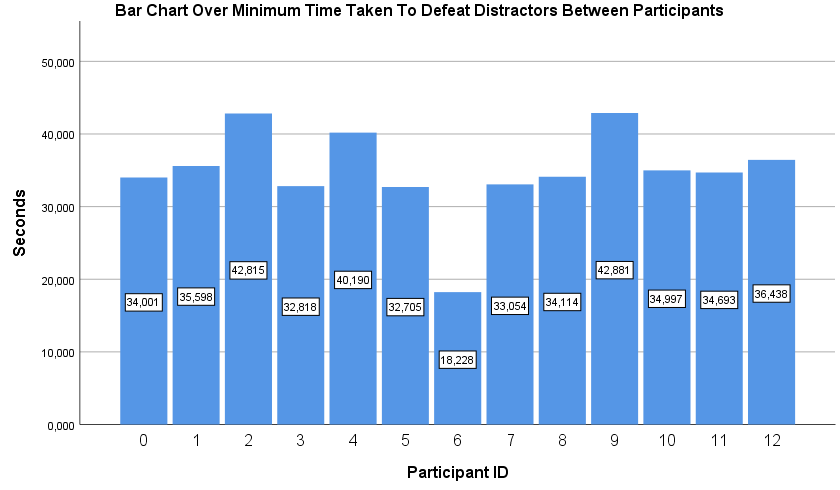
\includegraphics[width=0.75\textwidth]{figures/graphs/MinDistractorDefeatTime.png}
    \caption[Minimum Time Needed To Defeat Distractors Between Participants]{This bar chart shows the minimum time needed for each participant do defeat any distractor in Ensemble Retriever.}
    \label{fig:minDistractorDefeatTime}
\end{figure}

\subsubsection{Time/Walking Speed Normalisation}
* Two variables that potentially could have some effect on the the reset counts between conditions is the time spent on walking and the walking speed of participants. It is thus necessary to first look at the average movement speed and time spent on walking between the conditions. 

* Time Spent Walking is in Figure~\ref{fig:TimeSpentWalkingBetweenConditions}
\begin{figure}[tbph]
    \centering
    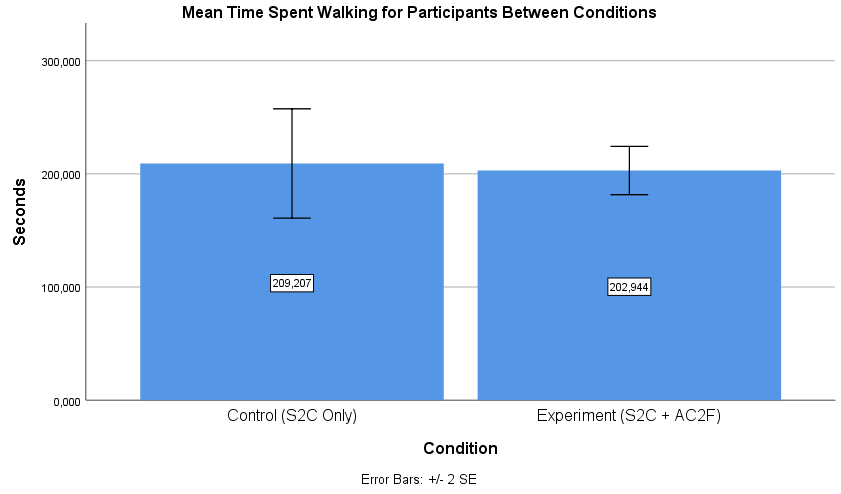
\includegraphics[width=0.75\textwidth]{figures/graphs/TimeSpentWalkingBetweenConditions.png}
    \caption[Mean Time Spent Walking Between Conditions]{This bar chart shows the mean time participants spent on walking between the two conditions.}
    \label{fig:TimeSpentWalkingBetweenConditions}
\end{figure}

* Mean Metres per Second between conditions is in Figure~\ref{fig:ex2mps}
\begin{figure}[tbph]
    \centering
    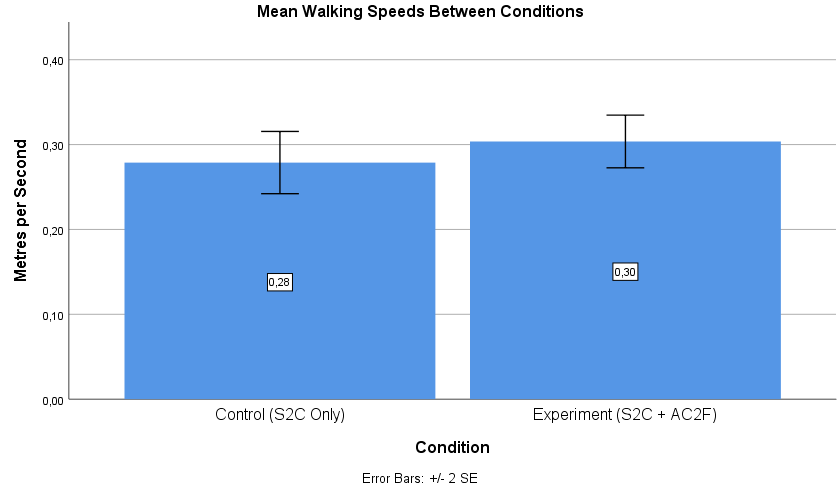
\includegraphics[width=0.75\textwidth]{figures/graphs/mpsBetweenConditions.png}
    \caption[Mean Walking Speed Between Conditions]{This bar chart shows the mean walking speed of participants between conditions.}
    \label{fig:ex2mps}
\end{figure}

* They are pretty similar.\todo{Do I need to do anything more with these two or are they similar enough that I only have to show that they are similar?}

\subsubsection{Mean Number of Resets for Participants Between Conditions}
* Figure~\ref{fig:ex2resetMeans}.
\begin{figure}[tbph]
    \centering
    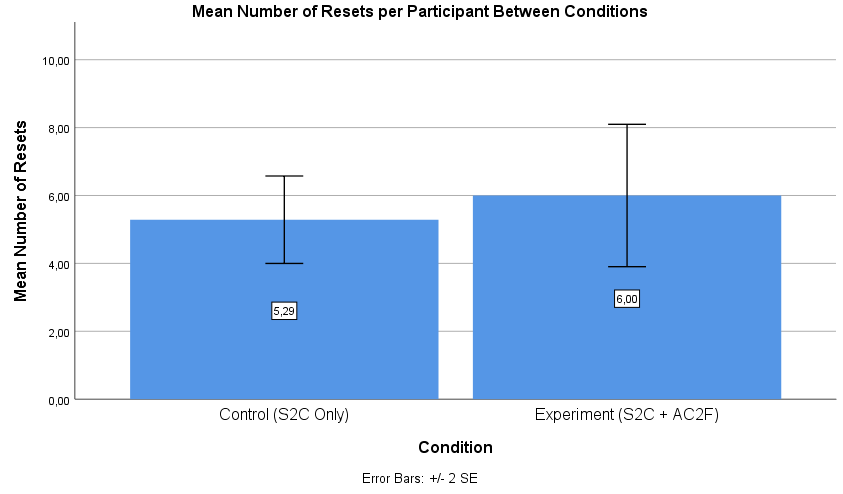
\includegraphics[width=0.75\textwidth]{figures/graphs/ResetMeans.png}
    \caption[Mean Number of Resets Between Conditions]{This bar chart shows the mean number of resets that participants experienced between conditions.}
    \label{fig:ex2resetMeans}
\end{figure}

\subsubsection{Hypothesis Testing}

\subsection{Alignment Time Effectiveness}